% document formatting
\documentclass[10pt]{article}
\usepackage[utf8]{inputenc}
\usepackage[left=1in,right=1in,top=1in,bottom=1in]{geometry}
\usepackage[T1]{fontenc}
\usepackage{xcolor}

% math symbols, etc.
\usepackage{amsmath, amsfonts, amssymb, amsthm}

% lists
\usepackage{enumerate}
\usepackage{enumitem}

% images
\usepackage{graphicx} % for images
\usepackage{tikz}
\usetikzlibrary{arrows.meta}

% code blocks
% \usepackage{minted, listings} 

% verbatim greek
\usepackage{alphabeta}

% custom commands
\newcommand{\rank}{\text{Rank}}
\newcommand{\select}{\text{Select}}

\graphicspath{{./assets/images/Week 11}}

\title{02-614 Week 11 \\ \large{String Algorithms}}
 
\author{Aidan Jan}

\date{\today}

\begin{document}
\maketitle
\section*{Text Editors}
How do text editors store strings?  This is an interesting question since when a file is opened in a text editor, it is assumed that the text contained in the file will change\dots a lot.  Previously, we were given a string which we assumed would be constant.  However, that is no longer the case, and many of the data structures already covered would not work since we don't have the ability to do preprocessing.

\subsection*{Data Structures}
\subsubsection*{Line-Oriented Data Structures}
The file is represented as a linked list with each node containing a linked list. 
\begin{itemize}
    \item This is efficient in inserting lines, since it just means creating a new node.
    \item However, it is suboptimal for inserting characters since we would have to iterate through the text.
    \item In the worst case, if the text file is a single, really long line, then this is just equivalent to the na\"ive way of storing a string.
\end{itemize}

\subsubsection*{Gap Buffer}
Imagine $T$ as an array, and create a buffer of some size after the cursor.
\begin{itemize}
    \item If we move the cursor, then copy the character after the buffer to the front.  The buffer does not change size with this operation.
    \item If we type, we begin to fill the buffer.
    \item The downside is if we fill up the buffer, we must copy the entire string to a new, larger array in order to create a new buffer.  Guessing an optimal buffer size becomes important.
\end{itemize}
This is the strategy Emacs uses.

\subsubsection*{Piece Tables}
Let $T$ be a series of text that is fixed (assumed to not change).  Let $M$ be an array (also text) that can grow.  Now, we represent the string as a table.
\begin{center}
\begin{tabular}{|c|c|c|}
    \hline
    T/M & P & length \\ \hline
    T & 0 & 10 \\
    M & 0 & 5 \\
    T & 11 & 5 \\
    M & 6 & 32 \\ \hline
\end{tabular}
\end{center}
To get a string, we read off of the table.  In this example, our string would be composed of characters $T[0:10] + M[0:5] + T[11:16] + M[6:38]$.
\begin{itemize}
    \item The benefit of this approach is that once we find the correct position in the table, inserting or deleting text happens in constant time.
    \begin{itemize}
        \item To insert, we split a row into two, the first one the section in $T$ we want to edit, and the second in $M$, containing our edit.
        \item To delete, split the row in $T$ into two rows in $T$, and just change the starting indices to slice the string.
    \end{itemize}
    \item When the file is saved, all the changes are written to $T$.
    \item The length of the table is never longer than the length of the string.  However, $M$ can grow in an unbounded manner if edits are large.
\end{itemize}
This is the basis of the strategy Code OSS (VS Code) uses.  More specifically, Code OSS uses their own designed ``piece trees''.

\subsubsection*{Ropes}
Consider the the string ``the quick brown fox''.  The Ropes strategy breaks it into a series of nodes (not necessarily separated by word boundaries).  One possible example may be [(the), ( qui), (ck), (brow), (n fox)].  Now, we make these nodes the leaf nodes of a binary tree.
\begin{center}
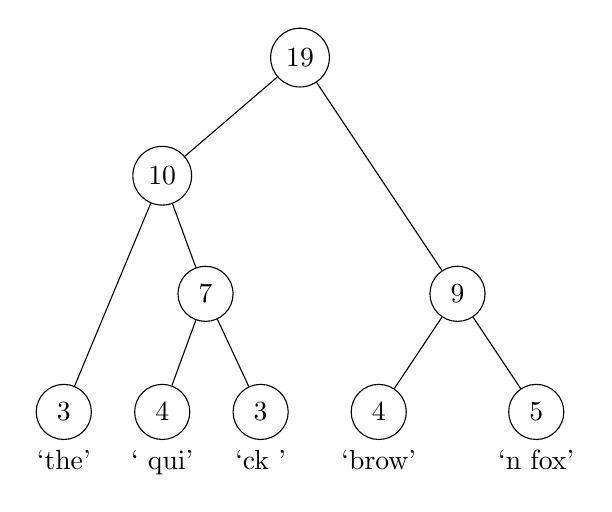
\begin{tikzpicture}
    \node[draw, circle, minimum size=0.7cm] at (0, 0) (0) {$19$};
    \node[draw, circle, minimum size=0.7cm] at (-1.75, -1.5) (1) {$10$};
    \node[draw, circle, minimum size=0.7cm] at (-1.2, -3) (2) {$7$};
    \node[draw, circle, minimum size=0.7cm] at (2, -3) (3) {$9$};
    \node[draw, circle, minimum size=0.7cm, label=below:`the'] at (-3, -4.5) (4) {$3$};
    \node[draw, circle, minimum size=0.7cm, label=below:` qui'] at (-1.75, -4.5) (5) {$4$};
    \node[draw, circle, minimum size=0.7cm, label=below:`ck '] at (-0.5, -4.5) (6) {$3$};
    \node[draw, circle, minimum size=0.7cm, label=below:`brow'] at (1, -4.5) (7) {$4$};
    \node[draw, circle, minimum size=0.7cm, label=below:`n fox'] at (3, -4.5) (8) {$5$};

    \draw (0) -- (1);
    \draw (0) -- (3);
    \draw (1) -- (2);
    \draw (1) -- (4);
    \draw (2) -- (5);
    \draw (2) -- (6);
    \draw (3) -- (7);
    \draw (3) -- (8);
\end{tikzpicture}
\end{center}
For the tree, we would use some balanced search tree (Splay, AVL, Red/Black).  Nodes store the number of characters represented.
\begin{itemize}
    \item To reconstruct the string, we read the data in an in-order traversal of the tree.
    \item To insert text, split the leaf to create a new node, and rebalance the tree.
    \item To delete text, edit the text in the nodes directly.
\end{itemize}





\end{document}